\documentclass[serif,mathserif]{beamer}
\usepackage{amsmath, amsfonts, epsfig, xspace}
\usepackage{algorithm,algorithmic}
\usepackage{pstricks,pst-node}
\usepackage{multimedia}
\usepackage[normal,tight,center]{subfigure}
\setlength{\subfigcapskip}{-.5em}
\usepackage{beamerthemesplit}
\usetheme{lankton-keynote}

\usepackage{color}
\usepackage{listings}
\definecolor{dkgreen}{rgb}{0,0.6,0}
\definecolor{gray}{rgb}{0.5,0.5,0.5}
\definecolor{mauve}{rgb}{0.58,0,0.82}

\lstset{frame=tb,
  language=C,
  aboveskip=3mm,
  belowskip=3mm,
  showstringspaces=false,
  columns=flexible,
  basicstyle={\small\ttfamily},
  numbers=none,
  numberstyle=\tiny\color{gray},
  keywordstyle=\color{green},
  commentstyle=\color{dkgreen},
  stringstyle=\color{mauve},
  breaklines=true,
  breakatwhitespace=true,
  tabsize=3
}

\author[Mohammad Mahzoun]{Mohammad Mahzoun}

\title[Low Level Security\hspace{2em}\insertframenumber/\inserttotalframenumber]{Buffer overflow}

\date{May 24, 2018} %leave out for today's date to be insterted

\institute{University of Tehran}

\begin{document}

\maketitle

% \section{Introduction}  % add these to see outline in slides

\begin{frame}
  \frametitle{Introduction}
  What is a buffer overflow?
  \begin{itemize}
  \item A buffer overflow is a bug that affects low-level code, typically written in C and
 C++, with significant security implications. 
 \item
 	A program with this bug will simply crash.
 	\item
 	But an Attacker can do much worse!
 	\begin{itemize}
 		\item
 			\textbf{Steal} private information.
 		\item
 			\textbf{Corrupt} valuable information.
 		\item
 			\textbf{Run} arbitrary code.
 			
 	\end{itemize}
 
  \end{itemize}
\end{frame}

% \section{Main Body} % add these to see outline in slides

\begin{frame}
  \frametitle{History}
  History of buffer overflows
  \begin{itemize}
  \item \textcolor{red}{Morris worm (1988)}
	\begin{itemize}
		\item 
			Propagated across the machines using buffer overflow.
		\item
			End result: \$10-100M in damages 
	\end{itemize}	  
  
  \item \textcolor{red}{CodeRed (2001)}
  	\begin{itemize}
		\item 
			Exploited an overflow in MS-IIS server 
		\item
			300,000 machines infected in 14 hours
	\end{itemize}
  \item \textcolor{red}{X11 Vulnerability (2014)}
  	\begin{itemize}
		\item 
			The bug was in code for more than 20 years.
	\end{itemize}
  \end{itemize}
\end{frame}

\begin{frame}
  \frametitle{History}
	\begin{center}
	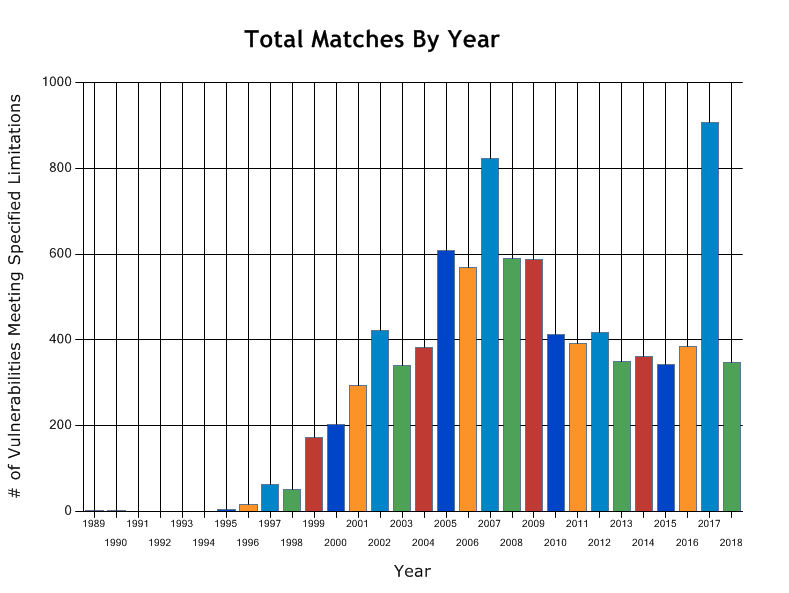
\includegraphics[width=9.5cm]{reports.png}
    \\
	https://nvd.nist.gov/vuln/search/statistics
	\end{center}
    
\end{frame}

\begin{frame}
  \frametitle{C memory layout}
  A typical memory representation of C program consists of following sections:
  \begin{itemize}
  	\item
  		Text segment
  		\begin{itemize}
  			\item  contains executable instructions.
  			\item  Placed below the heap or stack in order to prevent heaps and stack overflows from overwriting it.
		\end{itemize}  		 
	\item
		Initialized data segment
		\begin{itemize}
			\item
			virtual address space contains the global variables and static variables initialized.
			
		\end{itemize}
	\item Uninitialized Data Segment
		\begin{itemize}
			\item bss (block started by symbol) 
			\item all global variables and static variables that are initialized to zero or do not have explicit initialization
		\end{itemize}							
  \end{itemize}
\end{frame}

\begin{frame}
  \frametitle{C memory layout}
  A typical memory representation of C program consists of following sections:
  \begin{itemize}
  	\item Stack
  		\begin{itemize}
  			\item local variables variables
  			\item saved information after function calls
  		\end{itemize}
  	\item Heap
  		\begin{itemize}
  			\item begins at the end of the BSS segment and grows to larger addresses from there.
  			\item managed by malloc, realloc, and free, which may use the brk and sbrk system calls to adjust its size.
  		\end{itemize}
  \end{itemize}
\end{frame}

\begin{frame}
  \frametitle{C memory layout}
  \begin{center}
    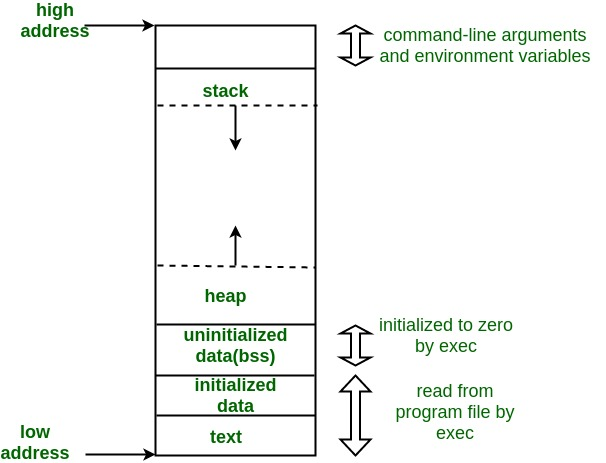
\includegraphics[scale=0.45]{memoryLayoutC.jpg}
  \end{center}

\end{frame}


% \section{Conclusion} % add these to see outline in slides

\begin{frame}
  \frametitle{Stack and function calls}
  \begin{itemize}
  	\item what happens when we call a function?
  		\begin{itemize}
  			\item what data needs to be stored?
  			\item where does it go?
  		\end{itemize}
  	\item what happens when we return from a function?
  		\begin{itemize}
  			\item what data needs to be restored?
  			\item where does come from?
  		\end{itemize}
  \end{itemize}
\end{frame}


\begin{frame}[fragile]
  \frametitle{Stack and function calls}
\begin{lstlisting}
void func(char* arg1, int arg2, int arg3)
{
    char loc1[4];
    int loc2;
    ...
}
\end{lstlisting}
\begin{center}
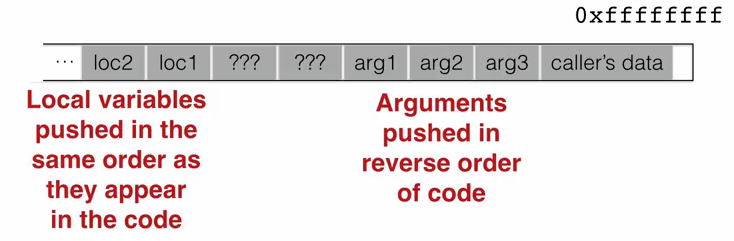
\includegraphics[scale=0.35]{stackff.png}
\end{center}

\end{frame}


\begin{frame}[fragile]
  \frametitle{Accessing variables}
\begin{lstlisting}
void func(char* arg1, int arg2, int arg3)
{
    ...
    loc2++; // Where is it? %ebp - 8
    ...
}
\end{lstlisting}
\begin{center}
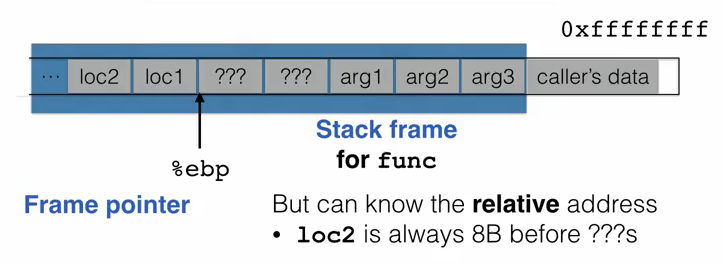
\includegraphics[scale=0.35]{stackff2.png}
\end{center}

\end{frame}

\begin{frame}[fragile]
  \frametitle{Returning from a function}
\begin{lstlisting}
int main()
{
    ...
    func("Hey", 10, -3);
    ...
}
\end{lstlisting}
\begin{center}
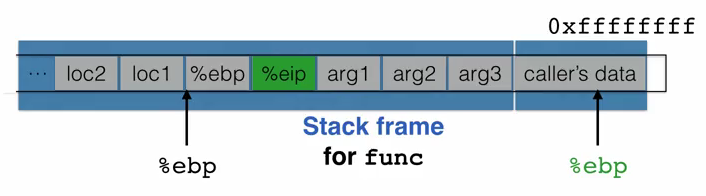
\includegraphics[scale=0.35]{stackff4.png}
\end{center}

\end{frame}



\begin{frame}[fragile]
  \frametitle{Returning from a function}

\end{frame}

\begin{frame}
  \frametitle{Questions}
\end{frame}
\end{document}
